% Block 1 of Day 1: Why inference moves to the edge.
%
% Topics of the syllabus: course overview; latency, bandwidth, privacy, cost,
% and availability; the cloud, edge, mobile, and TinyML paradigms; comparison
% of the two course boards with a typical Cortex-M4 microcontroller and with
% a cloud GPU. Exercise: select a paradigm for three applications.

% ------------------------------------------------------------ course overview
\begin{frame}{The course in three weeks}
  \small
  \renewcommand{\arraystretch}{1.25}
  \begin{tabular}{@{}L{0.07\textwidth}L{0.25\textwidth}L{0.19\textwidth}L{0.39\textwidth}@{}}
    \toprule
    \textbf{Week} & \textbf{Subject} & \textbf{Board} & \textbf{Days} \\
    \midrule
    1 & Foundations and TinyML & XIAOML Kit &
        Landscape, sensor data, model deployment, quantization, audio and
        vision \\
    2 & Optimization and Linux-class edge devices & Laptop, \mbox{Raspberry Pi 5} &
        Pruning and distillation, runtimes, object detection, benchmarking,
        generative AI \\
    3 & Connected systems and production & Both boards &
        RTSP streaming, MQTT, monitoring, production design, capstone \\
    \bottomrule
  \end{tabular}
  \vskip 1em
  \keypoint{You optimize a model, deploy it on two device classes, connect
    the devices, and monitor them. The capstone project combines all parts
    into one system.}
\end{frame}

\begin{frame}{How each day works}
  \begin{columns}[T]
    \begin{column}{0.47\textwidth}
      \begin{block}{Theory: three blocks}
        \begin{itemize}
          \item Block 1: the main concept of the day.
          \item Block 2: methods and tools.
          \item Block 3: design trade-offs and the lab briefing.
          \item Each block has one short exercise.
        \end{itemize}
      \end{block}
    \end{column}
    \begin{column}{0.47\textwidth}
      \begin{block}{Lab: groups of two students}
        \begin{itemize}
          \item You work on the hardware in two to four parts.
          \item You predict a number before you measure it.
          \item At the end you show the result to the instructor.
          \item You write a Decision Log.
        \end{itemize}
      \end{block}
    \end{column}
  \end{columns}
  \vskip 0.8em
  \begin{block}{Decision Log}
    A text of about 100 words. You state one design decision, you give the
    measured numbers, and you name the trade-off.
  \end{block}
\end{frame}

% ----------------------------------------------------------------------- terms
\begin{frame}{The terms of this course}
  \begin{columns}[c]
    \begin{column}{0.44\textwidth}
      \centering
      \begin{tikzpicture}[font=\footnotesize,
          ring/.style={rounded corners=6pt, line width=0.8pt}]
        \node[ring, draw=coolgray, minimum width=5.0cm, minimum height=4.6cm] (a) at (0,0) {};
        \node[ring, draw=darkcyan, minimum width=4.3cm, minimum height=3.5cm] (b) at (0,-0.4) {};
        \node[ring, draw=treegreen, minimum width=3.6cm, minimum height=2.4cm] (c) at (0,-0.8) {};
        \node[ring, draw=cardinalred, fill=boxgray, minimum width=2.6cm, minimum height=1.1cm]
          (d) at (0,-1.25) {\textbf{TinyML}};
        \node[anchor=north, text=coolgray] at (a.north) {Edge computing};
        \node[anchor=north, text=darkcyan] at (b.north) {Edge AI};
        \node[anchor=north, text=treegreen] at (c.north) {Embedded ML};
      \end{tikzpicture}
    \end{column}
    \begin{column}{0.54\textwidth}
      \small
      \begin{description}\itemsep 0.3em
        \item[Edge computing] Computation on a device at the edge of the
          network, near the data source.
        \item[Edge AI] A model makes the decision on the edge device.
        \item[Embedded ML] Inference on an embedded system. Training stays
          on a large computer.
        \item[TinyML] Inference on the smallest hardware: a microcontroller
          with kilobytes of memory.
      \end{description}
    \end{column}
  \end{columns}
  \source{\emph{XIAO: Big Power, Small Board}, chapter 4.1. Diagram drawn again
    for this course.}
\end{frame}

% ------------------------------------------------------------------- two paths
\begin{frame}{Two paths for inference}
  \centering
  \begin{tikzpicture}[font=\footnotesize, >={Stealth[length=5pt]},
      box/.style={draw=coolgray, rounded corners=3pt, minimum height=0.85cm,
                  minimum width=1.9cm, align=center, fill=boxgray},
      model/.style={box, draw=cardinalred, line width=0.8pt},
      lab/.style={font=\scriptsize, align=center, above}]
    % cloud path
    \node[anchor=west, text=coolgray] at (-0.95,0.85) {\textbf{Cloud path}};
    \node[box] (s1) at (0,0) {Sensor};
    \node[box] (n1) at (3.0,0) {Network};
    \node[model] (m1) at (6.0,0) {Model on\\a server};
    \node[box] (a1) at (9.0,0) {Action};
    \draw[->] (s1) -- node[lab]{raw\\data} (n1);
    \draw[->] (n1) -- (m1);
    \draw[->] (m1) -- node[lab]{result} (a1);
    % edge path
    \node[anchor=west, text=coolgray] at (-0.95,-1.25) {\textbf{Edge path}};
    \node[box] (s2) at (0,-2.1) {Sensor};
    \node[model] (m2) at (3.0,-2.1) {Model on\\the device};
    \node[box] (a2) at (6.0,-2.1) {Action};
    \node[box, dashed] (c2) at (9.0,-2.1) {Cloud\\(optional)};
    \draw[->] (s2) -- node[lab]{raw\\data} (m2);
    \draw[->] (m2) -- node[lab]{result} (a2);
    \draw[->, dashed] (a2) -- node[lab]{result\\only} (c2);
  \end{tikzpicture}
  \vskip 0.5em
  \raggedright
  \begin{itemize}
    \item Training needs much computation. It stays on large computers.
    \item Inference can move to the device. Then the device needs no
          permanent connection.
    \item The cloud path has three problems: raw data uses bandwidth, each
          transmission uses power, and the sensor must stay connected.
  \end{itemize}
  \source{\emph{XIAO: Big Power, Small Board}, chapter 4.1.}
\end{frame}

% ---------------------------------------------------------------- five reasons
\begin{frame}{Five reasons to move inference to the edge}
  \renewcommand{\arraystretch}{1.35}
  \begin{tabular}{@{}p{0.21\textwidth}p{0.72\textwidth}@{}}
    \toprule
    \textbf{Reason} & \textbf{The question that you ask} \\
    \midrule
    Latency      & How much time can pass between the input and the
                   response? \\
    Bandwidth    & How much data does the sensor make each second? Can the
                   connection carry it? \\
    Privacy      & Is the data permitted to leave the device? \\
    Cost         & What does each inference cost in the cloud? What does
                   each device cost? \\
    Availability & Must the system work when the network fails? \\
    \bottomrule
  \end{tabular}
  \vskip 0.8em
  \keypoint{One of these constraints usually decides. Find that constraint
    first.}
  \source{The five factors of Jeff Bier (``BLERP'': bandwidth, latency,
    economics, reliability, privacy), from \emph{XIAO: Big Power, Small
    Board}, chapter 4.1.}
\end{frame}

% --------------------------------------------------------------------- latency
\begin{frame}{Latency: the speed of light sets a minimum}
  \begin{columns}[T]
    \begin{column}{0.56\textwidth}
      \[
        t_{\min} = \frac{2 \times \text{distance}}{c_{\text{fiber}}}
      \]
      California to Virginia: 3600 km.
      \[
        t_{\min} \approx \frac{2 \times 3600\ \text{km}}{200\,000\ \text{km/s}}
                 = 36\ \text{ms}
      \]
      \begin{itemize}
        \item Software adds 60 to 150 ms.
        \item A cloud service needs 100 to 200 ms in total.
        \item A faster network does not change the 36 ms.
      \end{itemize}
    \end{column}
    \begin{column}{0.40\textwidth}
      \small
      \renewcommand{\arraystretch}{1.2}
      \begin{tabular}{@{}lr@{}}
        \toprule
        \textbf{Application} & \textbf{Budget} \\
        \midrule
        Vehicle braking & $<$ 10 ms \\
        Game rendering  & $<$ 16 ms \\
        Robot control   & $<$ 20 ms \\
        Voice response  & $<$ 200 ms \\
        Web search      & $<$ 500 ms \\
        \bottomrule
      \end{tabular}
    \end{column}
  \end{columns}
  \source{\emph{Machine Learning Systems}, Volume I, chapter 2 and its slide
    deck.}
\end{frame}

\begin{frame}{Latency: use a budget for the complete path}
  \begin{block}{Rule}
    If the budget is $X$ ms, no operation that needs more than $X$ ms can be
    on the path from the input to the response.
  \end{block}
  \vskip 0.4em
  Example: a camera gives 30 frames each second. The system must answer
  before the next frame: $1000 / 30 \approx 33$ ms.
  \vskip 0.6em
  \begingroup\centering
  \begin{tikzpicture}[font=\footnotesize, x=0.055cm, y=1cm]
    % scale: 1 unit = 1 ms
    \draw[->, coolgray] (0,-0.2) -- (200,-0.2) node[right] {ms};
    \foreach \t in {0,50,100,150} {
      \draw[coolgray] (\t,-0.2) -- (\t,-0.3) node[below] {\t};
    }
    % budget line
    \draw[cardinalred, line width=1pt, dashed] (33,-0.2) -- (33,2.2)
      node[above] {budget 33 ms};
    % cloud bar
    \fill[coolgray!60] (0,1.2) rectangle (36,1.8);
    \fill[coolgray!30] (36,1.2) rectangle (96,1.8);
    \draw[coolgray, dashed] (96,1.2) rectangle (186,1.8);
    \node at (18,1.5) {light};
    \node at (66,1.5) {software, minimum};
    \node at (141,1.5) {software, maximum};
    \node[anchor=east] at (-2,1.5) {Cloud};
    % edge bar
    \fill[treegreen!45] (0,0.2) rectangle (25,0.8);
    \node[anchor=west] at (37,0.5) {no network term: measure this time on the device};
    \node[anchor=east] at (-2,0.5) {Edge};
  \end{tikzpicture}\par\endgroup
  \source{Rule and cloud numbers: \emph{Machine Learning Systems}, Volume I,
    chapter 2. The length of the edge bar is an example, not a measured
    value.}
\end{frame}

% ------------------------------------------------------------------- bandwidth
\begin{frame}{Bandwidth: send the result, not the raw data}
  \begin{columns}[T]
    \begin{column}{0.47\textwidth}
      \begin{block}{A car with 8 cameras}
        \begin{itemize}
          \item 30 frames each second
          \item 2 MB for each frame
        \end{itemize}
        \[
          8 \times 30 \times 2\ \text{MB} = 480\ \text{MB/s}
        \]
        No mobile connection carries this data rate.
      \end{block}
    \end{column}
    \begin{column}{0.47\textwidth}
      \begin{block}{A microphone on a microcontroller}
        \begin{itemize}
          \item 16\,000 samples each second
          \item 2 bytes for each sample
        \end{itemize}
        \[
          16\,000 \times 2\ \text{B} = 32\ \text{kB/s}
        \]
        A keyword result is one short message.
      \end{block}
    \end{column}
  \end{columns}
  \vskip 0.8em
  \begin{itemize}
    \item A site with hundreds of cameras cannot send all video to the cloud.
    \item Each transmitted byte also uses energy. A radio is expensive for a
          battery device.
  \end{itemize}
  \source{Car example: slide deck of \emph{Machine Learning Systems}, Volume
    I, chapter 2. Camera sites and energy: \emph{XIAO: Big Power, Small
    Board}, chapter 4.1.}
\end{frame}

% --------------------------------------------------------------------- privacy
\begin{frame}{Privacy: the data stays on the device}
  \begin{columns}[T]
    \begin{column}{0.46\textwidth}
      \begin{itemize}
        \item Cameras and microphones record persons.
        \item Data in the cloud passes through networks and servers.
        \item Some data must stay on the site: patient data, images of a
              production line.
        \item An edge device sends only the result, or nothing.
      \end{itemize}
    \end{column}
    \begin{column}{0.50\textwidth}
      \footnotesize
      \renewcommand{\arraystretch}{1.3}
      \begin{tabular}{@{}lll@{}}
        \toprule
        \textbf{Paradigm} & \textbf{Privacy} & \textbf{The data} \\
        \midrule
        Cloud  & Low     & leaves the device \\
        Edge   & High    & stays on the site \\
        Mobile & High    & stays on the phone \\
        TinyML & Highest & stays in the sensor \\
        \bottomrule
      \end{tabular}
    \end{column}
  \end{columns}
  \vskip 0.8em
  \keypoint{More shared computation gives less privacy. Data that stays local
    cannot use the computation of a data centre.}
  \source{\emph{Machine Learning Systems}, Volume I, chapter 2 and its slide
    deck.}
\end{frame}

% ------------------------------------------------------- cost and availability
\begin{frame}{Cost and availability}
  \begin{columns}[T]
    \begin{column}{0.47\textwidth}
      \begin{block}{Cost}
        \begin{itemize}
          \item Cloud computation and communication cost money for each
                inference. Video is the most expensive.
          \item An edge device sends less data and uses less cloud
                computation.
          \item A microcontroller costs 1 to 10 USD for each unit.
          \item The edge has its own costs: hardware maintenance and
                device management.
        \end{itemize}
      \end{block}
    \end{column}
    \begin{column}{0.47\textwidth}
      \begin{block}{Availability}
        \begin{itemize}
          \item A cloud service stops when the connection stops.
          \item A device with a local model continues to work.
          \item Example: a door lock with face recognition must open for
                the family when the internet fails.
          \item On Day 12 you build a system that operates offline.
        \end{itemize}
      \end{block}
    \end{column}
  \end{columns}
  \source{\emph{XIAO: Big Power, Small Board}, chapter 4.1. Unit cost and edge
    costs: slide deck of \emph{Machine Learning Systems}, Volume I, chapter
    2.}
\end{frame}

% ----------------------------------------------------------------- three walls
\begin{frame}{Why not one paradigm for all applications?}
  \begingroup\centering
  \begin{tikzpicture}[font=\footnotesize, node distance=2.4mm,
      col/.style={line width=0.8pt, rounded corners=3pt, fill=boxgray},
      head/.style={font=\small\bfseries, text=white, rounded corners=3pt,
                   minimum width=3.4cm, minimum height=0.6cm, anchor=north},
      txt/.style={align=flush center, text width=3.1cm, inner sep=1pt},
      res/.style={txt, font=\footnotesize\bfseries}]
    % light barrier
    \draw[col, draw=darkcyan] (-1.7,0) rectangle (1.7,-4.6);
    \node[head, fill=darkcyan] (h1) at (0,0) {Light barrier};
    \node[txt, below=of h1] (a1) {Light in fiber travels about
      200\,000~km/s.};
    \node[txt, below=of a1] (b1) {California to Virginia and back: 36~ms
      minimum.};
    \node[res, text=darkcyan, below=of b1] {A response in 10~ms cannot use a
      distant server.};
    % power wall
    \draw[col, draw=cardinalred] (1.9,0) rectangle (5.3,-4.6);
    \node[head, fill=cardinalred] (h2) at (3.6,0) {Power wall};
    \node[txt, below=of h2] (a2) {The power grows with the third power of
      the clock frequency.};
    \node[txt, below=of a2] (b2) {Two times the frequency needs eight times
      the power.};
    \node[res, text=cardinalred, below=of b2] {A phone has 3 to 5~W. It
      cannot run a data-centre model.};
    % memory wall
    \draw[col, draw=treegreen] (5.5,0) rectangle (8.9,-4.6);
    \node[head, fill=treegreen] (h3) at (7.2,0) {Memory wall};
    \node[txt, below=of h3] (a3) {Computation grows 1.6 times each year.
      Memory bandwidth grows 1.2 times.};
    \node[txt, below=of a3] (b3) {To move data often costs more than to
      compute on it.};
    \node[res, text=treegreen, below=of b3] {A microcontroller has 256~KB of
      RAM.};
  \end{tikzpicture}\par\endgroup
  \vskip 0.3em
  \keypoint{These limits are physics. No optimization removes them. They
    make four paradigms.}
  \source{\emph{Machine Learning Systems}, Volume I, chapter 2 and its slide
    deck. Diagram drawn again for this course.}
\end{frame}

% -------------------------------------------------------------- four paradigms
\begin{frame}{Four deployment paradigms}
  \begingroup\centering
  \begin{tikzpicture}[font=\footnotesize, >={Stealth[length=5pt]},
      p/.style={line width=0.9pt, rounded corners=3pt, fill=boxgray,
                minimum width=2.35cm, minimum height=1.0cm, align=center}]
    \node[p, draw=darkcyan]    (c) at (0,0)    {\textbf{Cloud ML}\\data centres};
    \node[p, draw=treegreen]   (e) at (2.75,0) {\textbf{Edge ML}\\local computers};
    \node[p, draw=coolgray]    (m) at (5.5,0)  {\textbf{Mobile ML}\\smartphones};
    \node[p, draw=cardinalred] (t) at (8.25,0) {\textbf{TinyML}\\microcontrollers};
    \draw[->, coolgray] (9.4,0.85) -- node[above] {more computation, more
      memory, more power} (-1.15,0.85);
    \draw[->, coolgray] (-1.15,-0.85) -- node[below] {nearer to the data: less
      latency, more privacy, less dependence on the network} (9.4,-0.85);
  \end{tikzpicture}
  \vskip 0.5em
  \small
  \renewcommand{\arraystretch}{1.15}
  \setlength{\tabcolsep}{4.5pt}
  \begin{tabular}{@{}llllll@{}}
    \toprule
    \textbf{Paradigm} & \textbf{Memory} & \textbf{Power} & \textbf{Latency}
      & \textbf{Privacy} & \textbf{Network} \\
    \midrule
    Cloud  & 80 GB  & 700 W        & 100 to 1000 ms & Low     & Necessary \\
    Edge   & 32 GB  & 15 to 40 W   & 10 to 100 ms   & High    & Intermittent \\
    Mobile & 8 GB   & 3 to 5 W     & 5 to 50 ms     & High    & Optional \\
    TinyML & 256 KB & 100 mW       & 1 to 10 ms     & Highest & None \\
    \bottomrule
  \end{tabular}\par\endgroup
  \source{Table: slide deck of \emph{Machine Learning Systems}, Volume I,
    chapter 2. Each row gives one typical device of the class.}
\end{frame}

\begin{frame}{Cloud ML: maximum computation}
  \begin{columns}[T]
    \begin{column}{0.47\textwidth}
      \begin{block}{Strengths}
        \begin{itemize}
          \item Computation and storage grow with the demand.
          \item Very large data sets.
          \item Large models, for example large language models.
          \item Training of almost all models.
        \end{itemize}
      \end{block}
    \end{column}
    \begin{column}{0.47\textwidth}
      \begin{block}{Limits}
        \begin{itemize}
          \item Latency: each request crosses the network.
          \item The data leaves the device.
          \item The system needs a connection.
          \item The cost increases with each request.
        \end{itemize}
      \end{block}
    \end{column}
  \end{columns}
  \vskip 0.8em
  \keypoint{Use the cloud when the application accepts the latency, the data
    can leave the device, and the model needs the computation.}
  \source{\emph{Machine Learning Systems}, Volume I, chapter 2 and its slide
    deck.}
\end{frame}

\begin{frame}{Edge ML: computation near the data}
  \begingroup\centering
  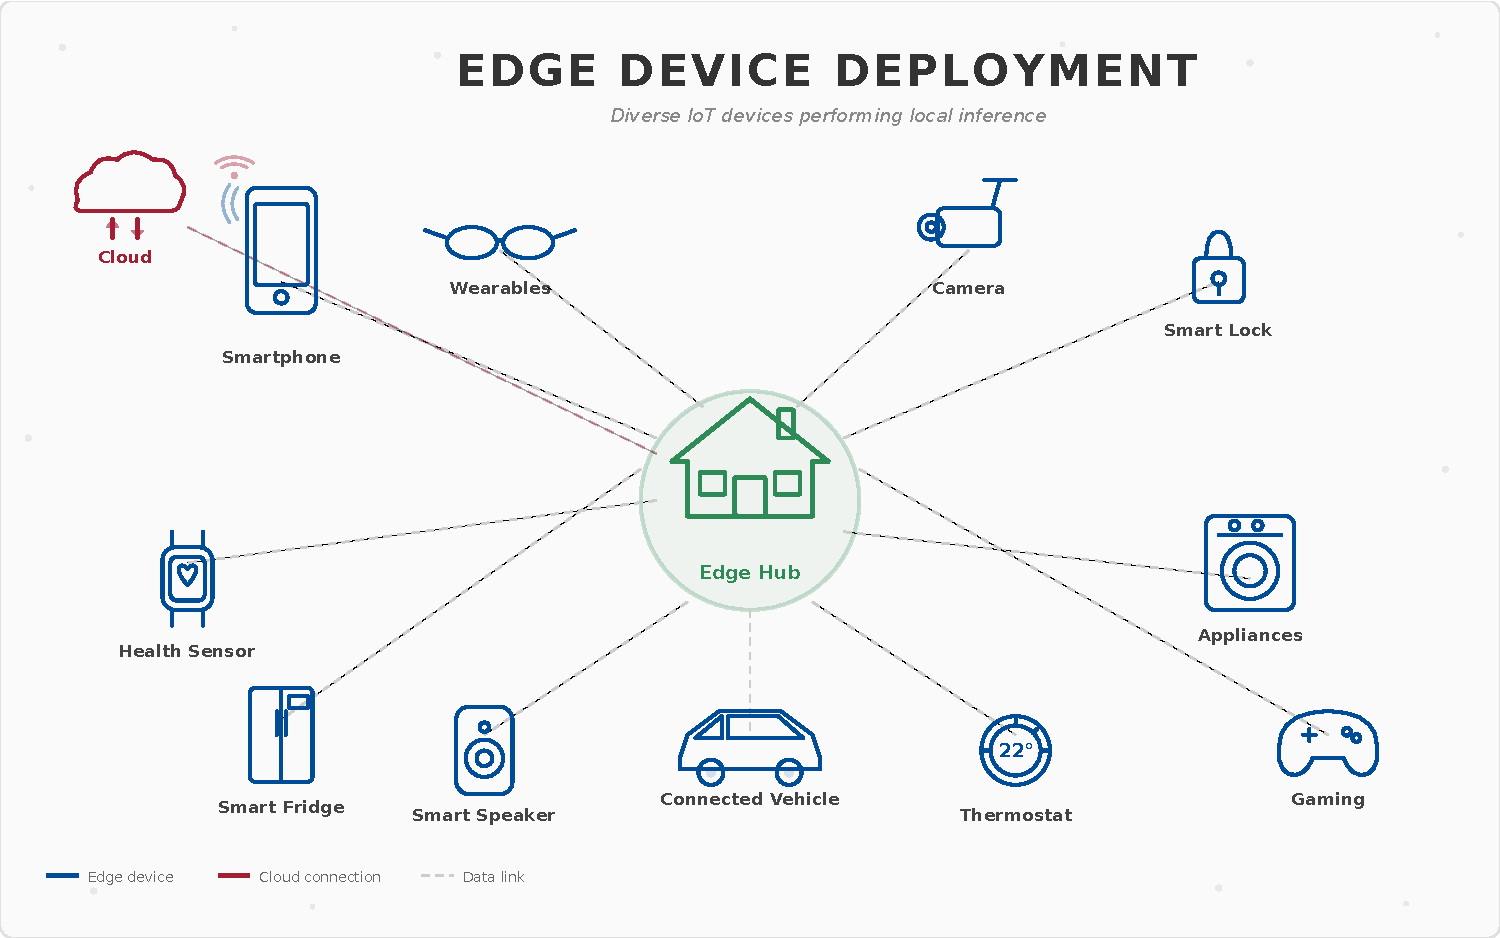
\includegraphics[height=4.3cm]{images/day01/edge-device-deployment.pdf}\par
  \endgroup
  \vskip 0.2em
  \small
  \begin{columns}[T]
    \begin{column}{0.47\textwidth}
      \begin{itemize}
        \item A local computer or a gateway runs the model. The data stays
              on the site.
        \item No round trip to a data centre.
      \end{itemize}
    \end{column}
    \begin{column}{0.47\textwidth}
      \begin{itemize}
        \item Limits: less computation than the cloud. You must maintain
              the hardware.
        \item \textbf{In this course:} the Raspberry~Pi~5.
      \end{itemize}
    \end{column}
  \end{columns}
  \source{Figure and text: \emph{Machine Learning Systems}, Volume I, chapter 2
    (CC BY-NC-SA 4.0).}
\end{frame}

\begin{frame}{Mobile ML: a battery and no fan}
  \begin{columns}[T]
    \begin{column}{0.53\textwidth}
      \begin{itemize}
        \item The model runs on a smartphone or a tablet.
        \item Advantages: it works offline, the data stays with the user,
              and the latency is low.
        \item The power limit is 3 to 5 W. The device has no fan.
        \item Above this limit the processor decreases its clock speed.
              Example: 60 frames each second decrease to 15 in one minute.
      \end{itemize}
    \end{column}
    \begin{column}{0.42\textwidth}
      \begin{block}{Battery calculation}
        A battery of 15 Wh:
        \begin{itemize}
          \item at 5 W: $15 / 5 = 3$ hours
          \item at 1 W: $15 / 1 = 15$ hours
        \end{itemize}
      \end{block}
    \end{column}
  \end{columns}
  \vskip 0.6em
  \keypoint{Mobile ML needs models that are designed for this limit, for
    example MobileNetV2. Block 2 shows why such a model costs less.}
  \source{\emph{Machine Learning Systems}, Volume I, chapter 2 and its slide
    deck.}
\end{frame}

\begin{frame}{TinyML: a different class, not a small phone}
  \begin{columns}[T]
    \begin{column}{0.50\textwidth}
      \small
      \renewcommand{\arraystretch}{1.25}
      \begin{tabular}{@{}lll@{}}
        \toprule
        & \textbf{Mobile} & \textbf{TinyML} \\
        \midrule
        Memory     & 8 GB     & 256 KB \\
        Power      & 3 to 5 W & 100 mW \\
        Parameters & millions & 10\,000 to 100\,000 \\
        \bottomrule
      \end{tabular}
      \vskip 0.6em
      Memory: a factor of about 30\,000.\\
      Power: a factor of 30 to 50.
    \end{column}
    \begin{column}{0.46\textwidth}
      \begin{itemize}
        \item The model runs on a microcontroller, next to the sensor.
        \item The device is always on. It can use a battery.
        \item The energy of each inference and the memory decide, not
              the speed.
        \item Example: a keyword spotting model has 26\,000 parameters and
              less than 100 KB.
      \end{itemize}
    \end{column}
  \end{columns}
  \vskip 0.4em
  \keypoint{You cannot make a mobile model smaller until it fits. TinyML
    needs different models and different tools.}
  \source{Slide deck of \emph{Machine Learning Systems}, Volume I, chapter 2.}
\end{frame}

% ---------------------------------------------------------- decision framework
\begin{frame}{How to select a paradigm}
  \begingroup\centering
  \begin{tikzpicture}[font=\footnotesize, >={Stealth[length=5pt]},
      f/.style={draw, line width=0.8pt, rounded corners=3pt, fill=boxgray,
                minimum width=6.8cm, minimum height=0.82cm, align=left,
                text width=6.4cm},
      r/.style={text=coolgray, align=left, text width=3.5cm, anchor=west}]
    \node[f, draw=coolgray, align=center] (s) at (0,0)
      {Start: cloud, edge, mobile, TinyML};
    \node[f, draw=cardinalred] (f1) at (0,-1.1)
      {\textbf{1. Privacy.} Must the data stay on the device?};
    \node[f, draw=darkcyan] (f2) at (0,-2.2)
      {\textbf{2. Latency.} Is the budget less than 10 ms?};
    \node[f, draw=treegreen] (f3) at (0,-3.3)
      {\textbf{3. Computation.} Is the model above 100 MB?};
    \node[f, draw=coolgray] (f4) at (0,-4.4)
      {\textbf{4. Cost.} Compare the total cost of the options.};
    \foreach \a/\b in {s/f1, f1/f2, f2/f3, f3/f4} { \draw[->] (\a) -- (\b); }
    \node[r] at (3.6,-1.1) {Yes: remove the cloud.};
    \node[r] at (3.6,-2.2) {Yes: remove cloud, edge.};
    \node[r] at (3.6,-3.3) {Yes: remove TinyML.};
    \node[r] at (3.6,-4.4) {Result: one paradigm.};
  \end{tikzpicture}\par\endgroup
  \vskip 0.3em
  \small
  Apply the filters in order. Each filter removes the paradigms that are
  not possible. The method does not start with the ``best'' paradigm.
  \source{The four filters: \emph{Machine Learning Systems}, Volume I,
    chapter 2 and its slide deck. Diagram drawn again for this course.}
\end{frame}

% ---------------------------------------------------------------- course boards
\begin{frame}{The two boards of this course}
  \begin{columns}[T]
    \begin{column}{0.47\textwidth}
      \centering
      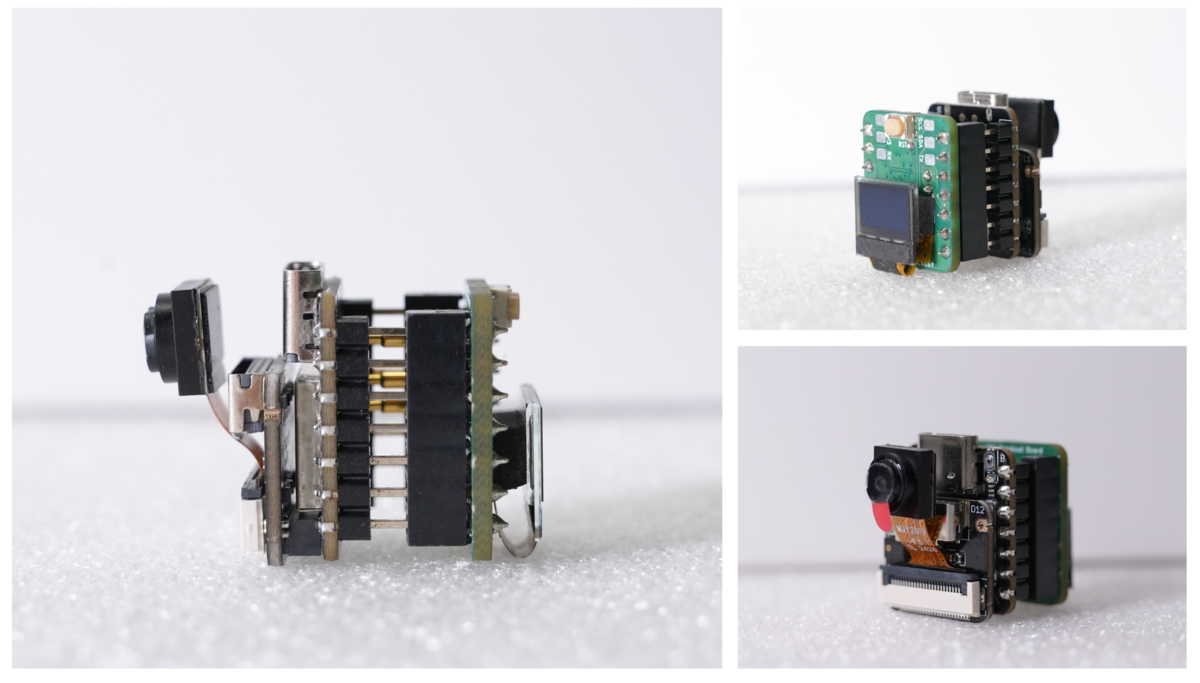
\includegraphics[height=2.3cm]{images/day01/xiaoml-kit.png}
      \vskip 0.3em
      \raggedright\small
      \textbf{XIAOML Kit} (TinyML)
      \begin{itemize}
        \item A microcontroller board with Wi-Fi and Bluetooth
        \item Camera, microphone, microSD card
        \item Expansion board: IMU and display
        \item Board size: 21 $\times$ 17.5 mm
      \end{itemize}
    \end{column}
    \begin{column}{0.47\textwidth}
      \centering
      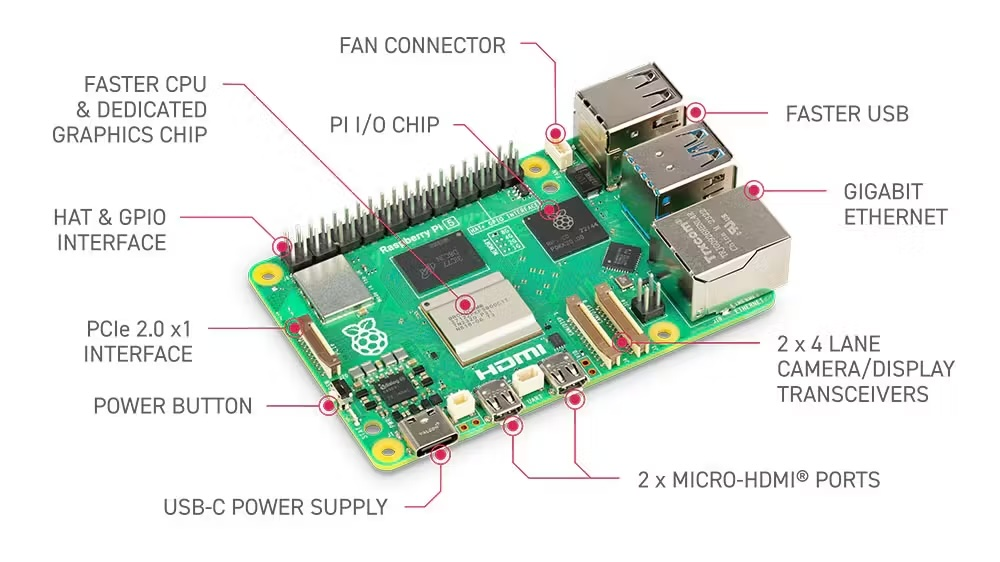
\includegraphics[height=2.3cm]{images/day01/raspberry-pi-5.jpg}
      \vskip 0.3em
      \raggedright\small
      \textbf{Raspberry Pi 5} (Edge ML)
      \begin{itemize}
        \item A single-board computer with 8 GB of RAM
        \item Linux, Python, complete ML frameworks
        \item Camera connector, USB, Ethernet, Wi-Fi
        \item With a camera and an active cooler
      \end{itemize}
    \end{column}
  \end{columns}
  \source{Photographs and data: kit pages of \emph{Machine Learning Systems}
    (CC BY-NC-SA 4.0).}
\end{frame}

\begin{frame}{Four devices, four budgets}
  \footnotesize
  \renewcommand{\arraystretch}{1.3}
  \setlength{\tabcolsep}{4pt}
  \begin{tabular}{@{}L{0.11\textwidth}L{0.20\textwidth}L{0.22\textwidth}L{0.20\textwidth}L{0.16\textwidth}@{}}
    \toprule
    & \textbf{Cortex-M4 microcontroller} & \textbf{XIAO ESP32S3 Sense}
    & \textbf{Raspberry Pi 5} & \textbf{Cloud GPU} \\
    \midrule
    Processor & Cortex-M4F, 1 core, 64 MHz
              & Xtensa LX7, 2 cores, 240 MHz
              & Cortex-A76, 4 cores, 2.4 GHz
              & GPU in a server \\
    RAM       & 256 KB & 512 KB, and 8 MB of PSRAM & 8 GB & 80 GB on the GPU \\
    Storage   & 1 MB of flash & 8 MB of flash & microSD card
              & Almost no limit \\
    Software  & Firmware in C++ & Firmware in C++, or MicroPython
              & Linux, Python & Linux, Python \\
    Paradigm  & TinyML & TinyML & Edge ML & Cloud ML \\
    \bottomrule
  \end{tabular}
  \vskip 0.6em
  \small
  The microcontroller column gives the nRF52840 of the Arduino Nano 33 BLE
  Sense. In the lab you build for the XIAO with PSRAM and with no PSRAM.
  \source{Kit pages and chapter 2 of \emph{Machine Learning Systems}; data
    sheets of the nRF52840 and of the ESP32-S3.}
\end{frame}

\begin{frame}{The memory of the four devices}
  \begingroup\centering
  \begin{tikzpicture}[font=\footnotesize, x=0.42cm, y=0.8cm]
    % x = log2(bytes) - 16. 256 KB = 2^18, 8 MB = 2^23, 8 GB = 2^33,
    % 80 GB = 2^36.3.
    \foreach \e/\l in {4/1 MB, 14/1 GB, 20/64 GB} {
      \draw[coolgray!50] (\e,-0.3) -- (\e,4.1);
      \node[below, coolgray] at (\e,-0.3) {\l};
    }
    \draw[->, coolgray] (0,-0.3) -- (22,-0.3) node[right] {RAM};
    \fill[cardinalred!70] (0,3.2) rectangle (2,3.8);
    \fill[cardinalred!40] (0,2.2) rectangle (7,2.8);
    \fill[treegreen!60]   (0,1.2) rectangle (17,1.8);
    \fill[darkcyan!60]    (0,0.2) rectangle (20.3,0.8);
    \node[anchor=west, fill=white, inner sep=1.5pt] at (2.3,3.5)  {Cortex-M4 microcontroller: 256 KB};
    \node[anchor=west, fill=white, inner sep=1.5pt] at (7.3,2.5)  {XIAO ESP32S3 with PSRAM: 8 MB};
    \node[anchor=west, text=white] at (0.3,1.5) {Raspberry Pi 5: 8 GB};
    \node[anchor=west, text=white] at (0.3,0.5) {Cloud GPU: 80 GB};
    \node[coolgray] at (11,4.3) {logarithmic scale: each step of the same
      length is the same factor};
  \end{tikzpicture}\par\endgroup
  \small
  \begin{itemize}
    \item From the microcontroller to the XIAO with PSRAM: a factor of 32.
    \item From the XIAO to the Raspberry Pi 5: a factor of about 1000.
    \item From the microcontroller to the cloud GPU: a factor of about
          300\,000.
  \end{itemize}
  \keypoint{A model that fits one device does not fit the next smaller
    device. You design the model for the target device.}
\end{frame}

% -------------------------------------------------------------------- exercise
\exerciseframe{select a paradigm}{%
  For each application, select one paradigm: cloud, edge, mobile, or TinyML.
  State the constraint that decides.
  \begin{enumerate}
    \item \textbf{A sensor on a water pipe in the desert.} It listens for the
          sound of a leak. It has a battery that must last one year. The site
          has no network connection.
    \item \textbf{A camera above a production line.} It must reject a
          defective part in 50 ms. The company does not permit the images to
          leave the factory. The model has a size of 200 MB.
    \item \textbf{A search tool for the document archive of a company.} It
          uses a large language model to answer questions. A user accepts an
          answer after two seconds.
  \end{enumerate}
  Work with your neighbour for 5 minutes. Use the four filters: privacy,
  latency, computation, cost.
}

\answerframe{select a paradigm}{%
  \begin{enumerate}
    \item \textbf{TinyML.} The energy decides: only a microcontroller
          operates for one year on a battery. Availability also removes the
          cloud, because the site has no connection.
    \item \textbf{Edge ML.} Privacy removes the cloud. The latency of 50 ms
          permits a local computer. The model of 200 MB removes TinyML. The
          camera has a fixed position and mains power, so a mobile device
          gives no advantage.
    \item \textbf{Cloud ML.} The computation decides: a large language model
          does not fit a small device. A latency of two seconds is
          acceptable. If the documents must stay in the company, the model
          runs on a server of the company.
  \end{enumerate}
  More than one constraint can apply. The filters remove the paradigms that
  are not possible.
}
